
\section{Results}
\label{sec:results}

\subsection{Paired evidence hiding increases UDR overall}

C0 FULL produces \CzeroUnsupported/\PtwoN unsupported decisions
(\CzeroUDR\%). C1 HIDDEN produces \ConeUnsupported/\PtwoN
(\ConeUDR\%). The paired risk difference is +\PrimaryRD{} percentage points with
95\% bootstrap CI [\PrimaryCILow,\PrimaryCIHigh] percentage points. The exact two-sided
McNemar test gives $p=1.8626451492309587\times10^{-9}$.

\begin{figure}[t]
\centering
% Frozen values from paper-values.tex.
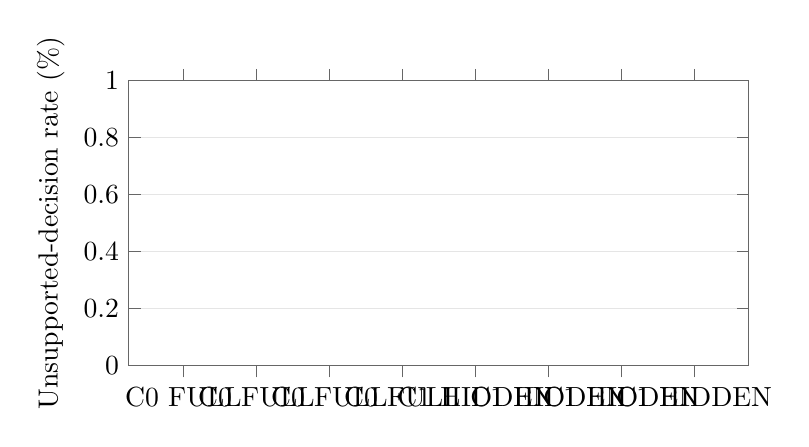
\begin{tikzpicture}
\begin{axis}[
  ybar,
  ymin=0, ymax=20,
  width=0.78\linewidth,
  height=5.2cm,
  ylabel={Unsupported-decision rate (\%)},
  symbolic x coords={C0 FULL,C1 HIDDEN},
  xtick=data,
  bar width=18pt,
  nodes near coords,
  nodes near coords align={vertical},
  enlarge x limits=0.35,
  ymajorgrids=true,
  grid style={black!10},
  axis line style={black!60},
  tick style={black!60},
  fill=black!22,
  draw=black
]
\addplot coordinates {(C0 FULL,\CzeroUDR) (C1 HIDDEN,\ConeUDR)};
\end{axis}
\end{tikzpicture}

\caption{\textbf{Paired evidence-visibility intervention.} World truth and the downstream
policy are fixed; only the designated mandatory item is hidden in C1. The aggregate effect
is heterogeneous across task families (Figure~\ref{fig:family}).}
\label{fig:primary}
\end{figure}

\subsection{The direct effect is concentrated in override/invalidation}

The aggregate effect hides extreme family heterogeneity. F1--F5 each remain at 0/30 UDR
under the direct C1 intervention, while F6 rises from 0/30 to 30/30.

\begin{figure}[t]
\centering
% Frozen direct-treatment family UDR.
\begin{tikzpicture}
\begin{axis}[
  ybar,
  ymin=0, ymax=105,
  width=\linewidth,
  height=5.8cm,
  ylabel={C1 UDR (\%)},
  symbolic x coords={F1,F2,F3,F4,F5,F6},
  xtick=data,
  bar width=15pt,
  nodes near coords,
  nodes near coords align={vertical},
  ymajorgrids=true,
  grid style={black!10},
  fill=black!22,
  draw=black
]
\addplot coordinates {
  (F1,\FoneCOne)
  (F2,\FtwoCOne)
  (F3,\FthreeCOne)
  (F4,\FfourCOne)
  (F5,\FfiveCOne)
  (F6,\FsixCOne)
};
\end{axis}
\end{tikzpicture}

\caption{\textbf{Direct-treatment heterogeneity.} F1--F5 retain a policy-visible gap cue
after the single designated item is removed and therefore trigger conservative fallback.
In F6, the later override/invalidation disappears completely while the older instruction
remains locally actionable. The 100\% F6 rate is a mechanism result for this frozen
policy--benchmark pair, not a real-world prevalence estimate.}
\label{fig:family}
\end{figure}

The direct experiment therefore does not support the statement that any missing mandatory
evidence is dangerous. It supports the narrower mechanism claim that an otherwise
conservative visible-gap policy can fail when superseding evidence disappears without
leaving a detectable trace.

\subsection{Frozen retrievers induce broader unsupported-decision patterns}

\begin{table}[t]
\centering
\small
\begin{tabular}{lrrrrr}
\toprule
Condition & Recall & Complete & UDR & Decisive & Safe decisive \\
\midrule
C0 FULL & 100.00 & 100.00 & 0.00 & 100.00 & 100.00 \\
C1 HIDDEN & 16.67 & 0.00 & 16.67 & 16.67 & 0.00 \\
C2 Lexical & \LexRecall & \LexCoverage & \LexUDR & \LexDecisive & \LexSafeDecisive \\
C3 Hash-dense & \HashRecall & \HashCoverage & \HashUDR & \HashDecisive & \HashSafeDecisive \\
C4 Hybrid & \HybridRecall & \HybridCoverage & \HybridUDR & \HybridDecisive & \HybridSafeDecisive \\
C5 Coverage-aware & \HybridRecall & \CoverageCoverage & \CoverageUDR & \CoverageDecisive & \CoverageSafeDecisive \\
\bottomrule
\end{tabular}
\caption{Aggregate P2 results, in percent. C1 required-fact recall is a mean over all
required facts; complete coverage is 0/180.}
\label{tab:aggregate}
\end{table}

Under C2--C4, UDR ranges from 29.44\% to 33.89\%. Top-$k$ retrieval can omit combinations
of evidence rather than exactly one preregistered target, and the family pattern broadens:
F1, F2, F4, and F6 show unsupported decisions under at least one frozen retriever.

\begin{table}[t]
\centering
\small
\begin{tabular}{lrrrr}
\toprule
Family & Lexical & Hash-dense & Hybrid & Coverage-aware \\
\midrule
F1 constraint & \FoneLex & \FoneHash & \FoneHybrid & 0 \\
F2 authority & \FtwoLex & \FtwoHash & \FtwoHybrid & 0 \\
F3 temporal & \FthreeLex & \FthreeHash & \FthreeHybrid & 0 \\
F4 conflict & \FfourLex & \FfourHash & \FfourHybrid & 0 \\
F5 outcome/revision & \FfiveLex & \FfiveHash & \FfiveHybrid & 0 \\
F6 override/invalidation & \FsixLex & \FsixHash & \FsixHybrid & 0 \\
\bottomrule
\end{tabular}
\caption{Family-level UDR (\%) for the retrieval conditions. Silentness is a property of
the resulting evidence surface relative to the policy, not a synonym for the F6 label.}
\label{tab:family-retrieval}
\end{table}

\subsection{Aggregate recall is not a strict monotonic safety surrogate}

Hash-dense yields 57.22\% mandatory-fact recall and 33.89\% UDR; hybrid yields 60.00\%
recall and 29.44\% UDR; lexical yields 63.06\% recall and 31.11\% UDR. The preregistered
directional gate passes within its 2 percentage-point tolerance, but strict monotonicity
fails: lexical has higher recall than hybrid and also 1.67 percentage points higher UDR.

\begin{figure}[t]
\centering
% Three frozen retrieval conditions only. No fitted line by design.
\begin{tikzpicture}
\begin{axis}[
  width=0.82\linewidth,
  height=5.6cm,
  xmin=55, xmax=65,
  ymin=27, ymax=36,
  xlabel={Mandatory-fact recall (\%)},
  ylabel={UDR (\%)},
  grid=both,
  grid style={black!10},
  axis line style={black!60},
  tick style={black!60}
]
\addplot[
  only marks,
  mark=*,
  mark size=3pt,
  black
] coordinates {
  (\HashRecall,\HashUDR)
  (\HybridRecall,\HybridUDR)
  (\LexRecall,\LexUDR)
};
\node[anchor=south west,font=\scriptsize] at (axis cs:\HashRecall,\HashUDR) {Hash-dense};
\node[anchor=north west,font=\scriptsize] at (axis cs:\HybridRecall,\HybridUDR) {Hybrid};
\node[anchor=south west,font=\scriptsize] at (axis cs:\LexRecall,\LexUDR) {Lexical};
\end{axis}
\end{tikzpicture}

\caption{\textbf{Aggregate recall is not a strict safety surrogate.} Three frozen
retrievers are shown without a fitted trend line. The data support a qualified directional
relationship, not a universal monotonic law.}
\label{fig:recall}
\end{figure}

Aggregate recall loses information about \emph{which} obligation disappeared and whether
the resulting absence is detectable by the downstream policy.

\subsection{Coverage awareness changes behavior on an identical surface}

C5 receives the identical retrieved evidence as C4 and only one additional bit indicating
whether all formal obligations are covered. C4 has UDR 53/180 = 29.44\%. C5 has UDR
0/180 while remaining decisive on all \HybridCompleteCount/\PtwoN cases with complete
formal coverage.

\begin{figure}[t]
\centering
% Same frozen retrieval surface: C4 and C5.
\begin{tikzpicture}
\begin{axis}[
  ybar,
  ymin=0, ymax=90,
  width=\linewidth,
  height=6.1cm,
  ylabel={Rate (\%)},
  symbolic x coords={UDR,Decisive,Safe decisive,Fallback},
  xtick=data,
  x tick label style={rotate=15,anchor=east},
  bar width=9pt,
  ymajorgrids=true,
  grid style={black!10},
  legend style={at={(0.5,1.02)},anchor=south,legend columns=2,draw=none}
]
\addplot[draw=black,fill=black!12] coordinates {
  (UDR,\HybridUDR)
  (Decisive,\HybridDecisive)
  (Safe decisive,\HybridSafeDecisive)
  (Fallback,\HybridFallback)
};
\addplot[draw=black,fill=black!48] coordinates {
  (UDR,\CoverageUDR)
  (Decisive,\CoverageDecisive)
  (Safe decisive,\CoverageSafeDecisive)
  (Fallback,\CoverageFallback)
};
\legend{C4 Hybrid,C5 Coverage-aware}
\end{axis}
\end{tikzpicture}

\caption{\textbf{Same-surface coverage-aware mitigation.} C4 and C5 share the identical
frozen hybrid retrieval surface (60.00\% mandatory-fact recall; 93/180 complete-coverage
cases). C5 adds only the completeness bit. Zero UDR here establishes sufficiency of this
information under the formal benchmark; it does not establish that a reliable coverage
signal is available in open-world deployment.}
\label{fig:coverage}
\end{figure}

C5 does not obtain zero UDR by refusing every case. Its decisive rate is 51.67\%, exactly
the 93 complete-coverage cases; the remaining 87 cases fall back. The result should be read
as a mechanism test: the downstream policy need not receive the missing evidence content
to avoid this measured failure, but it does need trustworthy information that an obligation
is uncovered.
